\documentclass{beamer}
\usepackage{hyperref}

\usetheme{Warsaw}

\title{Project Proposal: RF Controlled Relay Security Assessment}
\author{}
\date{}

\begin{document}

\begin{frame}
\titlepage
\end{frame}

\begin{frame}{Project Description}
We propose to assess the security of an RF controlled relay system operating at 433MHz. This project aims to evaluate the effectiveness of the claimed encryption between the remote control and the relay device. We will use a combination of hardware and software tools to capture RF traffic, attempt replay attacks, and investigate the possibility of a rolling key system. Our primary goals are to determine the reliability and robustness of the encryption mechanism and identify potential vulnerabilities in the system.
\end{frame}

\begin{frame}{Technology Stack}
\begin{itemize}
    \item Hardware:
    \begin{itemize}
        \item HackRF for RF signal capture \& transmission
        \item Yardstick One for signal capture \& transmission
        \item Remote Control Switch for messing with (kinda the whole point)
    \end{itemize}
    \item Software:
    \begin{itemize}
        \item GNU Radio for signal processing and analysis
        \item GQRX for visualization and monitoring
        \item Inspectrum for visualization and measurements
        \item Universal Radio Hacker for being lazy 
    \end{itemize}
    \item Operating System: Fedora Linux
\end{itemize}
\end{frame}

\begin{frame}{Timeline}
\begin{itemize}
    \item Week 1: Project setup, tool installation, and initial research
    \item Week 2: RF signal capture using HackRF and GQRX
    \item Week 3: Analyze captured data and attempt replay attacks
    \item Week 4: Investigate encryption mechanisms, likely rolling key, see if we can genirate a valid signal from hackrf/yardstick one
    \item Week 5: Finalize analysis, compile findings, and prepare the project report
\end{itemize}
\end{frame}

\begin{frame}{Responsibilities}
\begin{itemize}
    \item Catherine:
    \begin{itemize}
        \item Compile project report
        \item Initial data analysis
    \end{itemize}
    \item Louie:
    \begin{itemize}
       \item RF signal capture using HackRF and GQRX
        \item Research encryption mechanisms
    \end{itemize}
\end{itemize}
\end{frame}

\begin{frame}{Testing and Performance}
We will test the security of the RF controlled relay through a series of controlled experiments, including replay attacks and analysis of encryption mechanisms. Performance will be measured by the success or failure of these attacks and the identification of any security vulnerabilities.
\end{frame}

\begin{frame}{Challenges and Risks}
\begin{itemize}
    \item Encryption may prevent successful replay attacks.
    \item Attacking a rolling key system is complex and may not yield immediate results.
    \item Legal and ethical considerations related to RF signal interception.
\end{itemize}
\end{frame}

\begin{frame}{Ethical Considerations}
We will ensure responsible and legal use of tools and techniques throughout the project. We will obtain any necessary permissions for RF signal interception and adhere to ethical guidelines related to security research.
\end{frame}

\begin{frame}{Approvals}
This project proposal is subject to approval by the instructor.

\begin{center}
    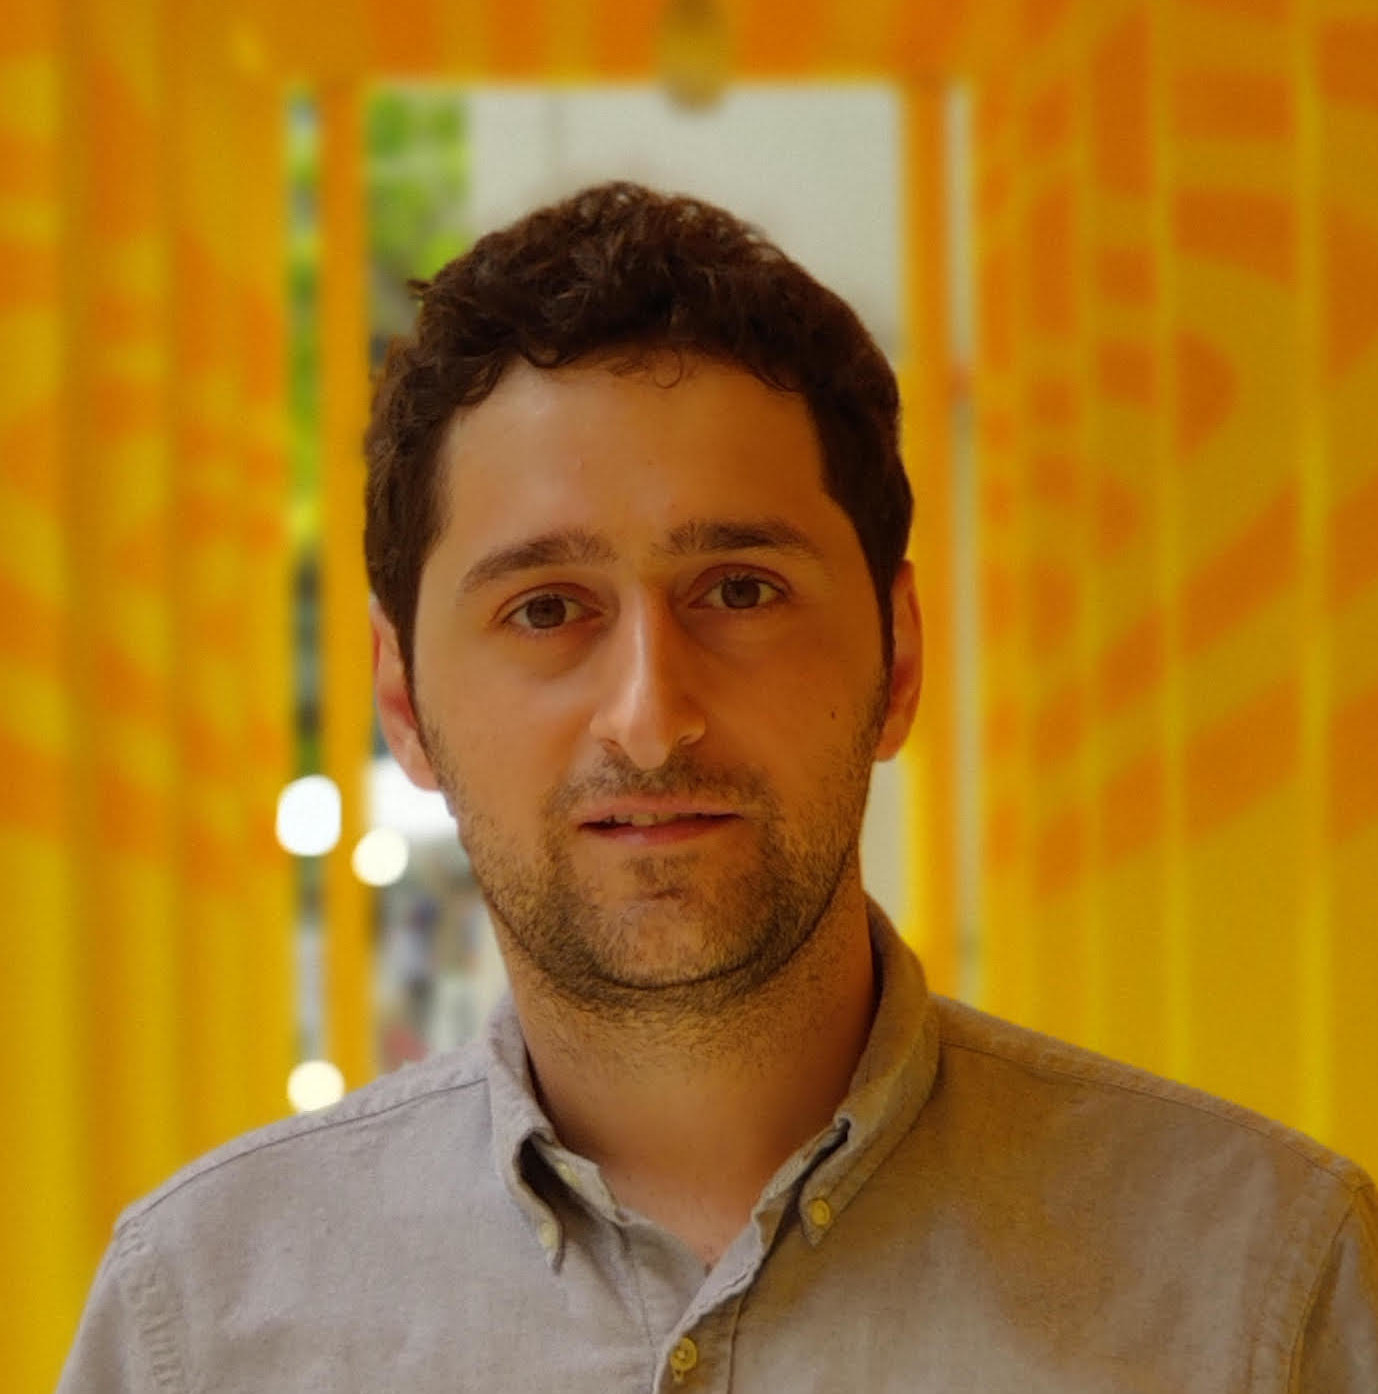
\includegraphics[width=0.6\linewidth]{./img/aydeger.jpeg}
\end{center}

\end{frame}

\begin{frame}{Documentation}
We will provide a project report in LaTeX format, covering system design, tool tutorials, and code documentation.

\begin{center}
    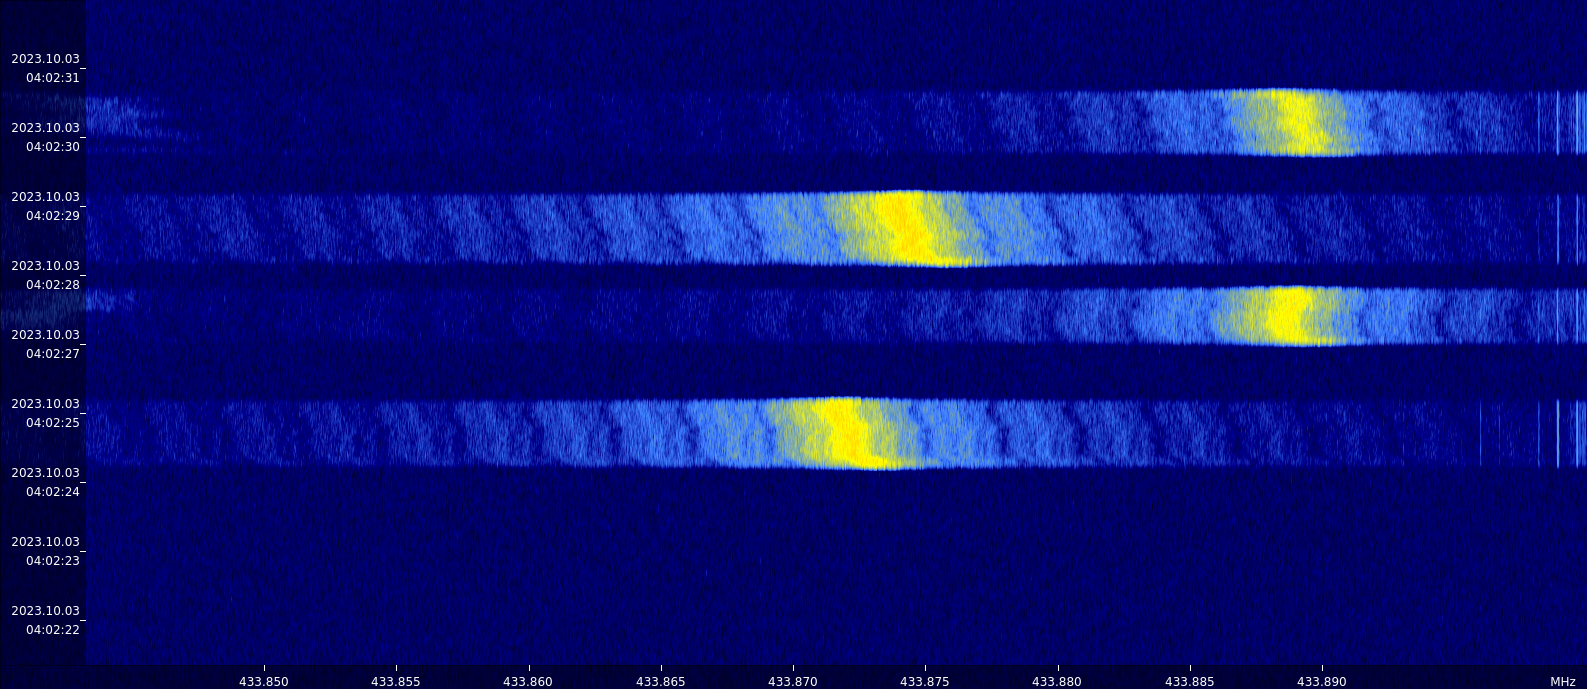
\includegraphics[width=0.9\linewidth]{./img/spec.png}
\end{center}


\end{frame}

\begin{frame}{Presentation}
We will deliver both a project proposal and a final project presentation in the class. \\ 
Help!\\
I'm trapped in a slideshow factory!\\
I've been stuck here since 1987!


\end{frame}

\begin{frame}{Additional Information}
A Picture of the device we are attacking\\
we could not think of more things to say, so here is a picture

\begin{center}
    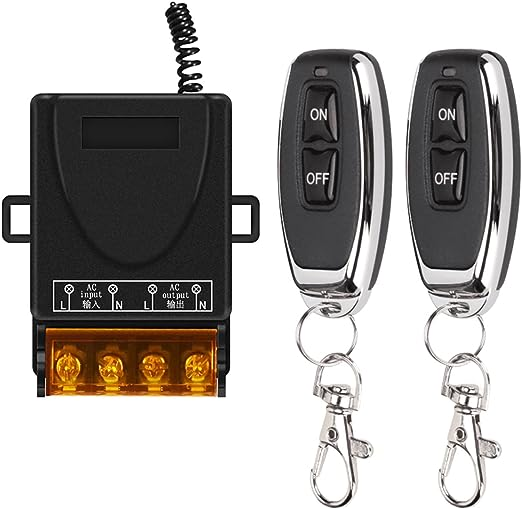
\includegraphics[width=0.6\linewidth]{./img/device.jpg}
\end{center}

\end{frame}


\begin{frame}{Any Questions}

\begin{center}
    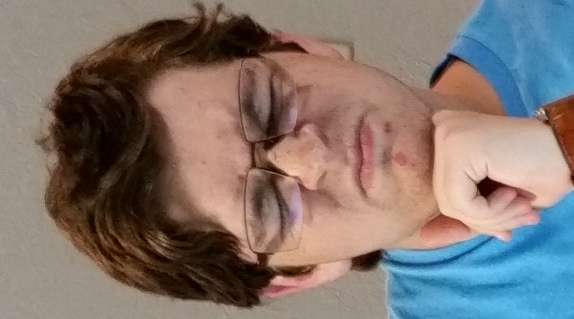
\includegraphics[width=1\linewidth]{./img/funny.jpg}
\end{center}

\end{frame}



\end{document}


